\documentclass[12pt, twoside]{article}
%\documentclass[12pt, twoside]{article}
\usepackage[letterpaper, margin=1in, headsep=0.2in]{geometry}
\setlength{\headheight}{0.6in}
%\usepackage[english]{babel}
\usepackage[utf8]{inputenc}
\usepackage{microtype}
\usepackage{amsmath}
\usepackage{amssymb}
%\usepackage{amsfonts}
\usepackage[nomessages]{fp} %\FPeval{\var-name}{2*sin(pi/6)}
\usepackage{siunitx} %units in math. eg 20\milli\meter
\usepackage{yhmath} % for arcs, overparenth command
\usepackage{tikz} %graphics
\usetikzlibrary{quotes, angles, arrows, arrows.meta}
\usepackage{pgfplots}
\usepgfplotslibrary{fillbetween}
\pgfplotsset{compat=1.16}
\usepackage{graphicx} %consider setting \graphicspath{{images/}}
\usepackage{parskip} %no paragraph indent
\usepackage{enumitem}
\usepackage{multicol}
\usepackage{venndiagram}

\usepackage{fancyhdr}
\pagestyle{fancy}
\fancyhf{}
\renewcommand{\headrulewidth}{0pt} % disable the underline of the header
\raggedbottom
\hfuzz=2mm %suppresses overfull box warnings

\usepackage{hyperref}

\fancyhead[LE]{\thepage}
\fancyhead[RO]{Markscheme}
\fancyhead[LO]{La Scuola d'Italia / Dr.\ Huson / IB Math 12 \\* 19 October 2026}

\begin{document}
\subsubsection*{2.1 Classwork: Right-Angled Triangle Trigonometry --- Markscheme}

\begin{enumerate}[itemsep=0.3cm]

%--- Problem 1: Name the sides; sin, cos, tan as fractions; angle from a ratio; side from sin; hypotenuse from cos [11 marks] ---
\item[1.] [Maximum mark: 11]

\textbf{(a)} hypotenuse $17$, opposite $15$, adjacent $8$ \hfill \textbf{A1A1}

\emph{A1 for the hypotenuse, A1 for both the opposite and the adjacent
sides. Accept the sides named by their vertices ($AB$, $BC$, $AC$) with
their lengths.}

\textbf{(b)} $\sin\theta = \frac{15}{17}$, \quad $\cos\theta = \frac{8}{17}$,
\quad $\tan\theta = \frac{15}{8}$ \hfill \textbf{A1A1A1}

\emph{FT from (a).}

\textbf{(c)} $\theta = \tan^{-1}\left(\frac{15}{8}\right)$ \hfill \textbf{M1}

$\theta = 61.9^\circ$ \quad ($61.9275\ldots$) \hfill \textbf{A1}

\emph{Accept $\sin^{-1}\left(\frac{15}{17}\right)$ or
$\cos^{-1}\left(\frac{8}{17}\right)$ for the M1. A value from a calculator
in radian mode ($1.08$) earns M1A0.}

\textbf{(d)} $\sin 35^\circ = \frac{QR}{12}$ \hfill \textbf{M1}

$QR = 12 \sin 35^\circ$

$QR = 6.88\,\text{cm}$ \quad ($6.88291\ldots$) \hfill \textbf{A1}

\textbf{(e)} $\cos 50^\circ = \frac{7}{x}$ \hfill \textbf{M1}

$x = \frac{7}{\cos 50^\circ}$

$x = 10.9$ \quad ($10.8900\ldots$) \hfill \textbf{A1}

\emph{The common error is $x = 7\cos 50^\circ = 4.50$, which treats $x$ as
the adjacent side: M0A0.}

\newpage

%--- Problem 2: Ladder (angle from cos, height); tower (elevation, height, hypotenuse, angle of depression) [10 marks] ---
\item[2.] [Maximum mark: 10]

\begin{minipage}[t]{0.68\linewidth}
\vspace{0pt}
\setlength{\parskip}{0.5\baselineskip}
\textbf{(a)} $\cos\theta = \frac{1.8}{6}$ \hfill \textbf{M1}

$\theta = 72.5^\circ$ \quad ($72.5423\ldots$) \hfill \textbf{A1}

\textbf{(b)} $h = 6 \sin 72.5423\ldots^\circ$ \hfill \textbf{M1}

$h = 5.72\,\text{m}$ \quad ($5.72363\ldots$) \hfill \textbf{A1}

\emph{Accept Pythagoras, $h = \sqrt{6^{2} - 1.8^{2}}$, for the M1. The
rounded angle gives the same value, $6 \sin 72.5^\circ = 5.72$. FT from (a).}
\end{minipage}
\hfill
\begin{minipage}[t]{0.28\linewidth}
\vspace{0pt}
\begin{tikzpicture}[scale=0.45]
  \coordinate (G) at (0,0);
  \coordinate (W) at (1.8,0);
  \coordinate (H) at (1.8,5.72);
  \draw[thick] (-0.5,0) -- (2.6,0);
  \draw[thick] (W) -- (1.8,6.4);
  \draw[very thick] (G) -- (H);
  \draw pic[draw, angle radius=0.2cm] {right angle = G--W--H};
  \draw pic["$\theta$", draw, angle radius=0.5cm, angle eccentricity=1.6] {angle = W--G--H};
  \node[below] at (0.9,0) {$1.8$};
  \node[left] at (0.9,2.86) {$6$};
  \node[right] at (1.8,2.86) {$h$};
\end{tikzpicture}
\end{minipage}

\textbf{(c)} $\tan 28^\circ = \frac{BT}{40}$ \hfill \textbf{M1}

$BT = 40 \tan 28^\circ$

$BT = 21.3\,\text{m}$ \quad ($21.2683\ldots$) \hfill \textbf{A1}

\textbf{(d)} $\cos 28^\circ = \frac{40}{PT}$ \hfill \textbf{M1}

$PT = \frac{40}{\cos 28^\circ}$

$PT = 45.3\,\text{m}$ \quad ($45.3028\ldots$) \hfill \textbf{A1}

\emph{Accept $\sin 28^\circ = \frac{BT}{PT}$, or Pythagoras
$PT = \sqrt{40^{2} + BT^{2}}$, for the M1. FT from (c).}

\textbf{(e)} angle of depression $=$ angle $TCB$ (alternate angles)

$\tan\alpha = \frac{21.2683\ldots}{60}$ \hfill \textbf{M1}

$\alpha = 19.5^\circ$ \quad ($19.5180\ldots$) \hfill \textbf{A1}

\emph{Accept $19.5^\circ$ from $\tan^{-1}\left(\frac{21.3}{60}\right) =
19.544\ldots$. FT from (c). The common error is the angle $BTC$ at the
top of the tower, $70.5^\circ$: M1A0.}

\end{enumerate}
\end{document}
